% ============================================================
% SECTION IV: METHODOLOGY -- restructured to match the existing paper.
% (Data preparation stays in Section III-D; it is NOT repeated here.)
%
% Subsection order:
%   A. Model Configuration
%   B. QLoRA Fine-Tuning Procedure   (equations 1-3 + Table IV)
%   C. Evaluation Framework          (equations 4-6)
%
% Citations appear ONLY on equations:
%   Eq. (1) LoRA [13], Eq. (2) QLoRA [10], Eq. (6) SSIM [28]
% [28] is the one NEW reference to append (bibitem at the bottom).
%
% No RTX 3070 Ti / 8 GB hardware references anywhere in this section.
% ============================================================

\section{Methodology}

The proposed methodology is a three-stage pipeline: (i)~construction and
preparation of the extended dataset (Section~III), (ii)~parameter-efficient
fine-tuning of the base model with QLoRA, and (iii)~automated evaluation along
code-level, visual-fidelity, and efficiency dimensions. Given a UI screenshot
as input, each model is asked to generate HTML with Tailwind CSS, a React JSX
component, and a Vue~3 SFC using identical task-specific prompts.
Fig.~\ref{fig:pipeline} illustrates the overall workflow.

\begin{figure}[!t]
\centering
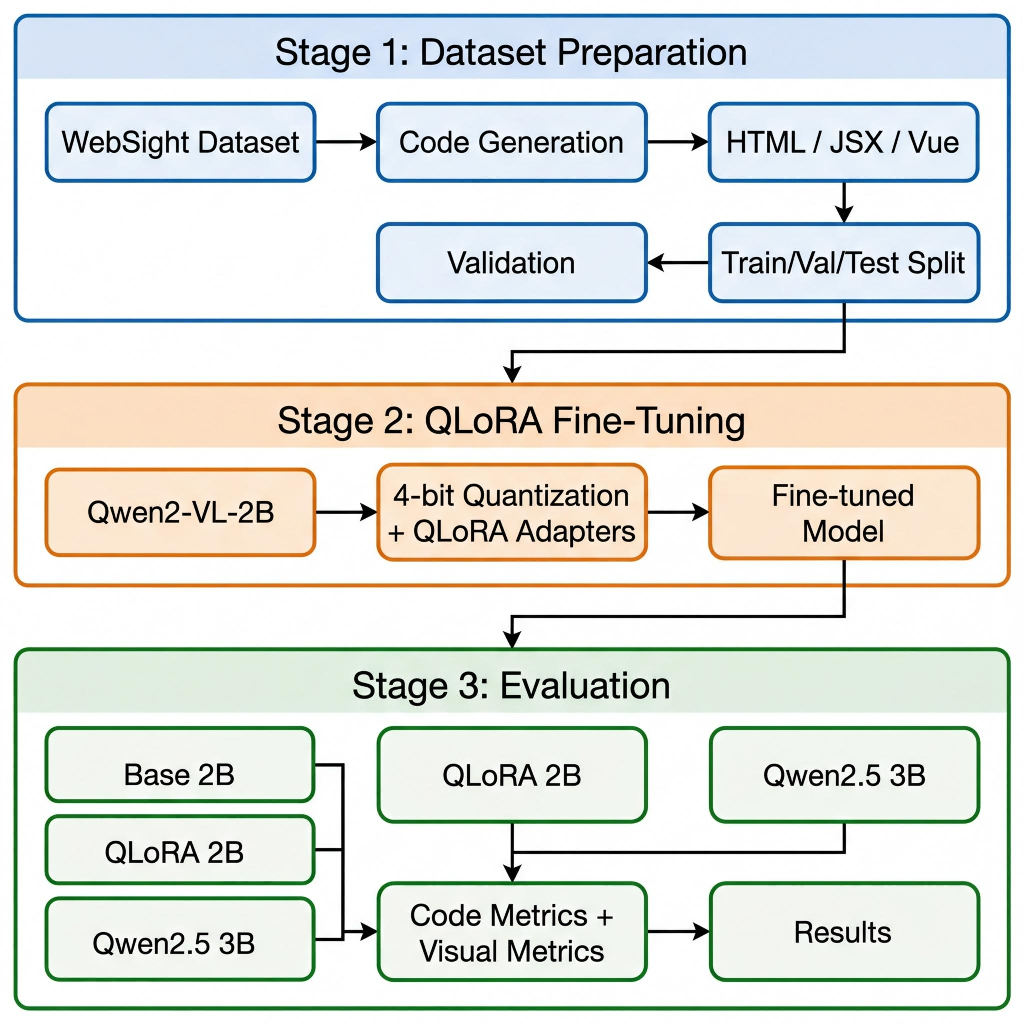
\includegraphics[width=\linewidth]{methodology_diagram_simple.pdf}
\caption{Proposed Pipeline.}
\label{fig:pipeline}
\end{figure}

\subsection{Model Configuration}

Three configurations are compared in order to isolate the effect of
parameter-efficient adaptation from the effect of scale:
\begin{itemize}
    \item \textbf{Qwen2-VL-2B-Instruct (Base):} the 2B-parameter
    vision-language model, evaluated zero-shot;
    \item \textbf{Qwen2-VL-2B-Instruct + QLoRA:} the same backbone fine-tuned
    on the extended dataset with QLoRA;
    \item \textbf{Qwen2.5-VL-3B-Instruct (Base):} a newer, larger 3B model,
    evaluated zero-shot to test whether scale alone can match task-specific
    adaptation.
\end{itemize}
All models receive identical prompts, the same visual-token budget, and
identical decoding: greedy decoding (no sampling) with a maximum of 1{,}536
new tokens per generation, which covers the length of the overwhelming
majority of reference outputs. Inference uses batched generation with
memory-efficient (SDPA/FlashAttention) attention kernels.

\subsection{QLoRA Fine-Tuning Procedure}

QLoRA combines 4-bit quantization of the frozen base weights with trainable
low-rank adapters. Following LoRA, the update to a pretrained weight matrix
$W_0 \in \mathbb{R}^{d \times k}$ is constrained to a low-rank decomposition
\begin{equation}
h \;=\; W_0 x \;+\; \Delta W x \;=\; W_0 x \;+\; \frac{\alpha}{r} B A x
\quad \cite{hu2021lora},
\label{eq:lora}
\end{equation}
where $A \in \mathbb{R}^{r \times k}$ and $B \in \mathbb{R}^{d \times r}$ are
the only trainable matrices, $r \ll \min(d,k)$ is the adapter rank, and
$\alpha$ is a scaling factor. In QLoRA the frozen weights are stored in 4-bit
NormalFloat (NF4) with double quantization and dequantized on the fly during
the forward pass:
\begin{equation}
h \;=\; \mathrm{dequant}\!\left(c^{(1)}, c^{(2)}, W^{\mathrm{NF4}}\right) x
\;+\; \frac{\alpha}{r}\, B A x \quad \cite{dettmers2023qlora},
\label{eq:qlora}
\end{equation}
where $c^{(1)}, c^{(2)}$ are the first- and second-level quantization
constants. Adapters of rank $r{=}64$ with $\alpha{=}128$ and dropout $0.05$
are attached to all attention and feed-forward projections (\texttt{q\_proj},
\texttt{k\_proj}, \texttt{v\_proj}, \texttt{o\_proj}, \texttt{gate\_proj},
\texttt{up\_proj}, \texttt{down\_proj}); the adapters are trained in FP16 while
the backbone remains frozen in NF4.

Training minimizes the causal language-modeling loss computed \emph{only} on
the assistant's code tokens. With image $I$, prompt $p$, and reference code
$y = (y_1, \dots, y_T)$, the objective is
\begin{equation}
\mathcal{L}(\theta) \;=\; -\sum_{t \in \mathcal{T}_{\mathrm{code}}}
\log p_\theta\!\left(y_t \,\middle|\, y_{<t},\, I,\, p\right),
\label{eq:loss}
\end{equation}
where $\mathcal{T}_{\mathrm{code}}$ indexes the assistant tokens; image and
prompt positions are excluded from the loss by label masking, so the model
learns code generation without altering its visual-encoder representations.
The model is trained on 25,215 multi-task examples (three tasks per image) for
3 epochs, with a validation pass over the 2,964 validation examples after the
final step. Table~\ref{tab:qlora_hyper} lists the hyperparameters.

\begin{table}[!t]
\centering
\caption{QLoRA Fine-Tuning Hyperparameters}
\label{tab:qlora_hyper}
\renewcommand{\arraystretch}{1.15}
\begin{tabular}{ll}
\hline
\textbf{Parameter} & \textbf{Value} \\
\hline
Base model            & Qwen2-VL-2B-Instruct \\
Quantization          & 4-bit NF4 (double quant.) \\
LoRA rank ($r$)       & 64 \\
LoRA alpha ($\alpha$) & 128 \\
LoRA dropout          & 0.05 \\
Learning rate         & $1 \times 10^{-4}$ \\
Warmup steps          & 100 \\
Weight decay          & 0.01 \\
Batch size            & 1 ($\times 8$ accum.) \\
Epochs                & 3 \\
Max sequence length   & 2{,}048 \\
Optimizer             & AdamW \\
Precision             & FP16 adapters, NF4 base \\
\hline
\end{tabular}
\end{table}

\subsection{Evaluation Framework}

All three models are evaluated on the 1,488 held-out test conversations.
Metrics are computed per task (HTML, JSX, Vue) and then averaged, so that no
task dominates the aggregate. Three complementary dimensions are measured.

\subsubsection{Code-Level Metrics}
Parse Success Rate (PSR) measures executable syntactic validity as the
fraction of generated outputs accepted by a production-grade parser
(\texttt{@babel/parser} for JSX, \texttt{@vue/compiler-sfc} for Vue):
\begin{equation}
\mathrm{PSR} \;=\; \frac{1}{N} \sum_{i=1}^{N}
\mathbb{1}\!\left[\,\mathrm{parse}(\hat{y}_i) = \text{success}\,\right].
\label{eq:psr}
\end{equation}
Similarity to the reference code is measured by BLEU-4, its code-aware
extension CodeBLEU (which adds AST-match and data-flow components), ROUGE-L,
ChrF, METEOR, and BERTScore~F1. Character-level closeness is captured by edit
similarity based on the Levenshtein distance $\mathrm{Lev}(\cdot,\cdot)$:
\begin{equation}
\mathrm{EditSim}(\hat{y}, y) \;=\;
1 - \frac{\mathrm{Lev}(\hat{y}, y)}{\max\!\left(|\hat{y}|, |y|\right)} .
\label{eq:editsim}
\end{equation}
Structure is assessed by tag accuracy (the fraction of reference HTML/JSX tags
recovered in the prediction), tree edit similarity---Eq.~\eqref{eq:editsim}
applied to the sequences of markup tags rather than characters---and
token-level accuracy, the fraction of aligned tokens that match exactly.

\subsubsection{Visual-Fidelity Metrics}
Each generated component is rendered in a headless Chromium browser
(Playwright) at a 1280$\times$960 viewport: raw HTML is wrapped in a full page
with Tailwind, JSX is mounted as a React component, and the Vue template is
extracted and rendered. The screenshot of the render is compared against the
original WebSight screenshot. Structural similarity is computed as
\begin{equation}
\mathrm{SSIM}(u,v) \;=\;
\frac{(2\mu_u \mu_v + C_1)(2\sigma_{uv} + C_2)}
     {(\mu_u^2 + \mu_v^2 + C_1)(\sigma_u^2 + \sigma_v^2 + C_2)}
\quad \cite{wang2004ssim},
\label{eq:ssim}
\end{equation}
with local means $\mu$, variances $\sigma^2$, covariance $\sigma_{uv}$, and
stabilization constants $C_1, C_2$. PSNR is reported as
$10\log_{10}(\mathrm{MAX}^2/\mathrm{MSE})$ in dB, and perceptual similarity by
LPIPS computed from deep AlexNet features, where lower is better. Samples whose
code fails to render are scored zero, so visual scores jointly reflect
renderability and appearance.

\subsubsection{Efficiency Metrics}
Inference latency is the wall-clock generation time averaged per sample under
batched inference, and memory cost is the peak allocated GPU memory (GiB)
recorded during inference. Together these determine deployability on
consumer-grade hardware.

% ============================================================
% ONE new reference to append (used by Eq. (6)):
% \bibitem{wang2004ssim} Z. Wang, A. C. Bovik, H. R. Sheikh, and
%   E. P. Simoncelli, ``Image quality assessment: from error visibility to
%   structural similarity,'' IEEE Trans. Image Process., vol. 13, no. 4,
%   pp. 600--612, 2004.
% ============================================================
